\section{E-commerce Overview}
\label{sec:e_commerce_overview}
As already mentioned, “E-Commerce is the activity of buying and selling of goods and services, especially on a large scale. Today, most of the population, use these virtual stores to shop or simply to inquire. In fact, these systems allow for a timely basis to have information regarding the good we are seeking. In this way these systems help the customer in buying a particular good.”
\newline
\begin{figure}[htb]
 \centering
 
\includegraphics[width=0.8\linewidth]{images/chapter1/e-commerce.png}\hfill
 \caption[e-commerce overview]{e-commerce overview}
 \label{fig:e_commerce_overview}
\end{figure}
The e-commerce in Europe has continued to grow even if at different rates and in different ways in different countries. Online shopping is a habit well established in Britain, Germany and France, markets that together account for 70-80\% of e-commerce Europe, while it is just starting out or is growing in the rest of Europe, including countries such as Italy and Spain. The most rapid growth, however, affect the emerging economies of Eastern Europe, led by Russia, the market for which is expected to grow by up to 200\% over the next three years.
\newline
In mature markets, growth was driven primarily by an increase in the frequency of purchase by the consumer and by the tendency to spend more through online channels, while in countries where e-commerce is developing growth results especially by the increase in online shoppers[2].
\begin{figure}[htb]
 \centering
 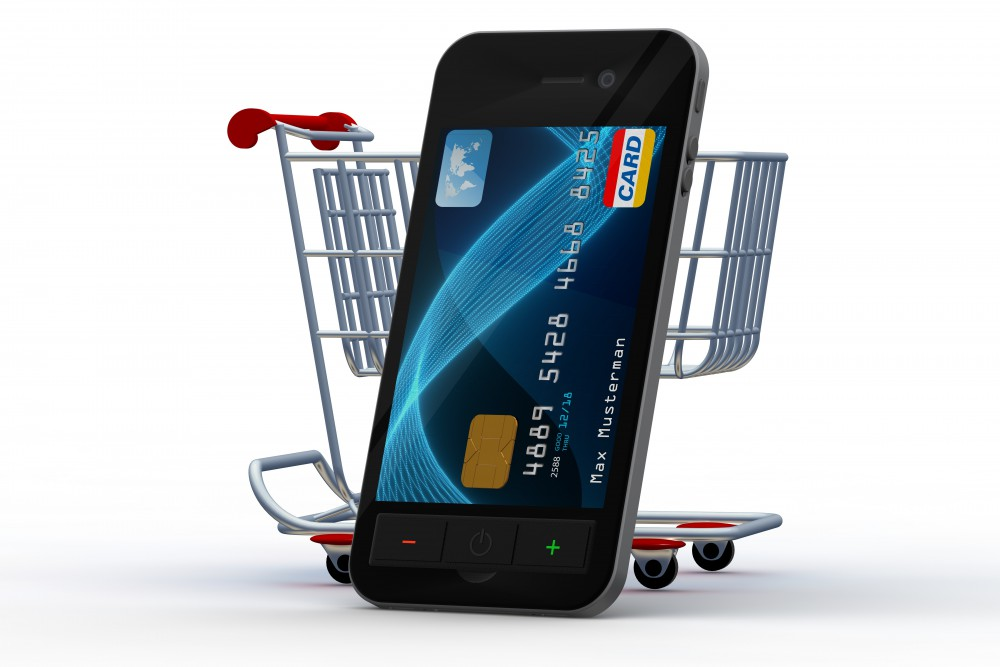
\includegraphics[width=1.0\linewidth]{images/chapter1/mobile-e-commerce.jpg}\hfill
 \caption[e-commerce payment system]{e-commerce payment system}
 \label{fig:e_commerce_mobile_system}
\end{figure}
The cabinet is the key factor in the growth of e-commerce. The diffusion of smartphones and tablets has extended much access to the online market, even in Italy, where 29 million end users access the Internet from the mobile. Companies that have not addressed this change have had a decline in the conversion rate on its website, while those who understood the new opportunities brought by the new type of access has been able to develop the offer of additional products and services dedicated, for example taking advantage of the geolocation of the customer. New entrants are mainly the physical stores, which saw in e-commerce for a way to expand its customer base, and producers of goods and services, they see the distribution companies increasingly as an obstacle to profitability.
What are the advantages and disadvantages (risks) of a system of e-commerce?
\newline
\subsection{Advantages and disadvantages of a system of e-commerce}
The benefits of electronic commerce are general (system-wide) and specific for the seller or the buyer.
\begin{itemize}
  \item Benefits for system:
  \begin{itemize}
    \item It is a global phenomenon and that a potentially global market;
    \item the transactions can develop throughout the day without interruption and realtime;
    \item the interaction between the parties can be synchronous or asynchronous;
    \item there is greater operational flexibility of relations between the parties.
  \end{itemize}

  \item Benefits for buyer:
  \begin{itemize}
    \item amenity: e-commerce stores are always open every day including holidays: just a few clicks from home or from work to buy what you want. The convenience to receive the goods directly at home is an important added value: we forget the long lines in the parking lot and in front of the chest of the crowded malls and you live a better buying experience;
    \item convenience: a purchase through the Web is much more convenient. In addition to the discounts and promotions who flock the network there is convenience in movement (no need to move by car or public services) and in the time saved;
    \item information: buying on the Internet allows you to calmly assess the choice of major purchases due to the large amount of information that you can easily find, to the advice and comments from other consumers, the wide range of products and alternatives;
  \end{itemize}
  \item Benefits for seller:
    \begin{itemize}
    \item the flexibility according to your needs of its commitments is easy to plan a few hours each day to devote to a new major project sales with the Internet. The mailbox collects communications and orders will be processed as soon as possible;
    \item visibility: there is no place in the world frequented the Internet, after an initial phase of advertising the same managers are surprised of the amount of visits and contacts received. Those who already have a business and want to open a new sales channel with the Internet, should not overlook the excellent positive return in terms of image that the site produces and that also benefits traditional activity;
    \item the economy: starting a new project sales with Internet does not require large investments and for the creation of storefront, both for advertising, both for the organization. Furthermore a good design e-commerce based on appropriate contacts with the suppliers allows to reduce to a minimum investment of stock.
  \end{itemize}\ldots
\end{itemize}
Companies that sell products or services on the Internet to be successful must obtain credibility and visibility on the Web and to achieve this it is not enough to have a secure server. To get credibility companies need to know how to build for the users of their website, a positive experience not only during the purchasing process, but also before and after, so that the user wants to repeat the experience and advice to other users. Creating a positive experience for their customers and by advertising messages and techniques of SEO companies build a reputation or image of successful enterprise.
In face-to-face transactions, customers and sellers use a number of physical signals to determine that they are dealing with a trustworthy partner. Retailers can check signatures and identity cards of their clients; buyers can see the badges with the name of employees, try the goods carefully and retain proof of their purchases. On electronic networks, none of these methods is applicable. For this reason, have been developed (and are now fully available and effective) some control systems performing similar functions.
The low cost of entry and the ease with which text and graphics can be copied, make it possible for almost anyone to create a website that pairs represent an organization established trading. No new reports of false virtual shops look professional, created to impersonate the Web version of existing activities, in order to illegally obtain credit card numbers. This problem has been resolved. Scammers are able to intercept transmissions. A thief can work hard to get the numbers of credit cards. A competitor or a disgruntled customer can enter an error in the company's website, in order to induce him to refuse service to potential customers or initiate other unauthorized actions. Sources intentional or accidental sometimes cause changes to the content of a communication route. User's name, credit card numbers and total currency are all vulnerable to such alteration. To this we have been developed safety systems to ensure the integrity of all the phases of the transaction. The data coming from America, are explicit: the continued growth of e-commerce is comforting. A concern, however, is the security front. In fact, the problems related to information security are increasing.
\newline
You can identify two types of Internet attacks to the network:
\begin{itemize}
  \item Passive attacks: Need to get the most information about the network in question, but does not have the purpose of hostile intrusion; (Ex. Eavesdropping: sniffing the information being sent across it in order to acquire the contents of transactions for subsequent analysis on personal data, or on behalf of third parties);
  \item Active attacks: as a result of the information collected by passive attacks, you can attack systems identified to implement changes to the data, lock services, obtain confidential information.\ldots
\end{itemize}
Another worrying phenomenon, in terms of information security, is
surely the phishing; It is an illegal system to collect sensitive data such as information about your credit card or access to bank accounts. The vast majority of messages takes place starting from phishing e-mail addresses stolen (ie where the authors have introduced illegally) or forged to perfection (in the eyes of the end user) on the basis of a known syntax or through the use of imitators sites of companies-mirror. These threats can cause a loss of integrity of databases, a loss of profits, increased costs for security systems, a critical data loss, a loss of trade secret information and damage to corporate reputation.
Systems e-commerce are the most famous Amazon, Ebay, etc..

\subsection{Amazon}
Amazon.com, Inc., often referred to as simply Amazon, is an American electronic commerce and cloud computing company with headquarters in Seattle,Washington. It is the largest Internet-based retailer in the United States. Amazon.com started as an online bookstore, later diversifying to sell DVDs, Blu-rays, CDs, videodownloads/streaming, MP3 downloads/streaming, audiobook downloads/streaming, software, video games, electronics, apparel, furniture, food, toys and jewelry. The company also produces consumer electronics—notably, Amazon Kindle e-book readers, Fire tablets, Fire TV and Fire Phone - and is the world's largest provider of cloud infrastructure services (IaaS). Amazon also sells certain low-end products like USB cables under its in-house brand AmazonBasics.
\newline
Amazon has separate retail websites for United States, United Kingdom and Ireland, France, Canada, Germany, Italy, Spain, Netherlands, Australia, Brazil, Japan, China, India and Mexico.
\newline
Amazon also offers international shipping to certain other countries for some of its products. In 2011, it professed an intention to launch its websites in Poland and Sweden.
In 2015, Amazon surpassed Walmart as the most valuable retailer in the United States by market capitalization.
\begin{figure}[htb]
 \centering
 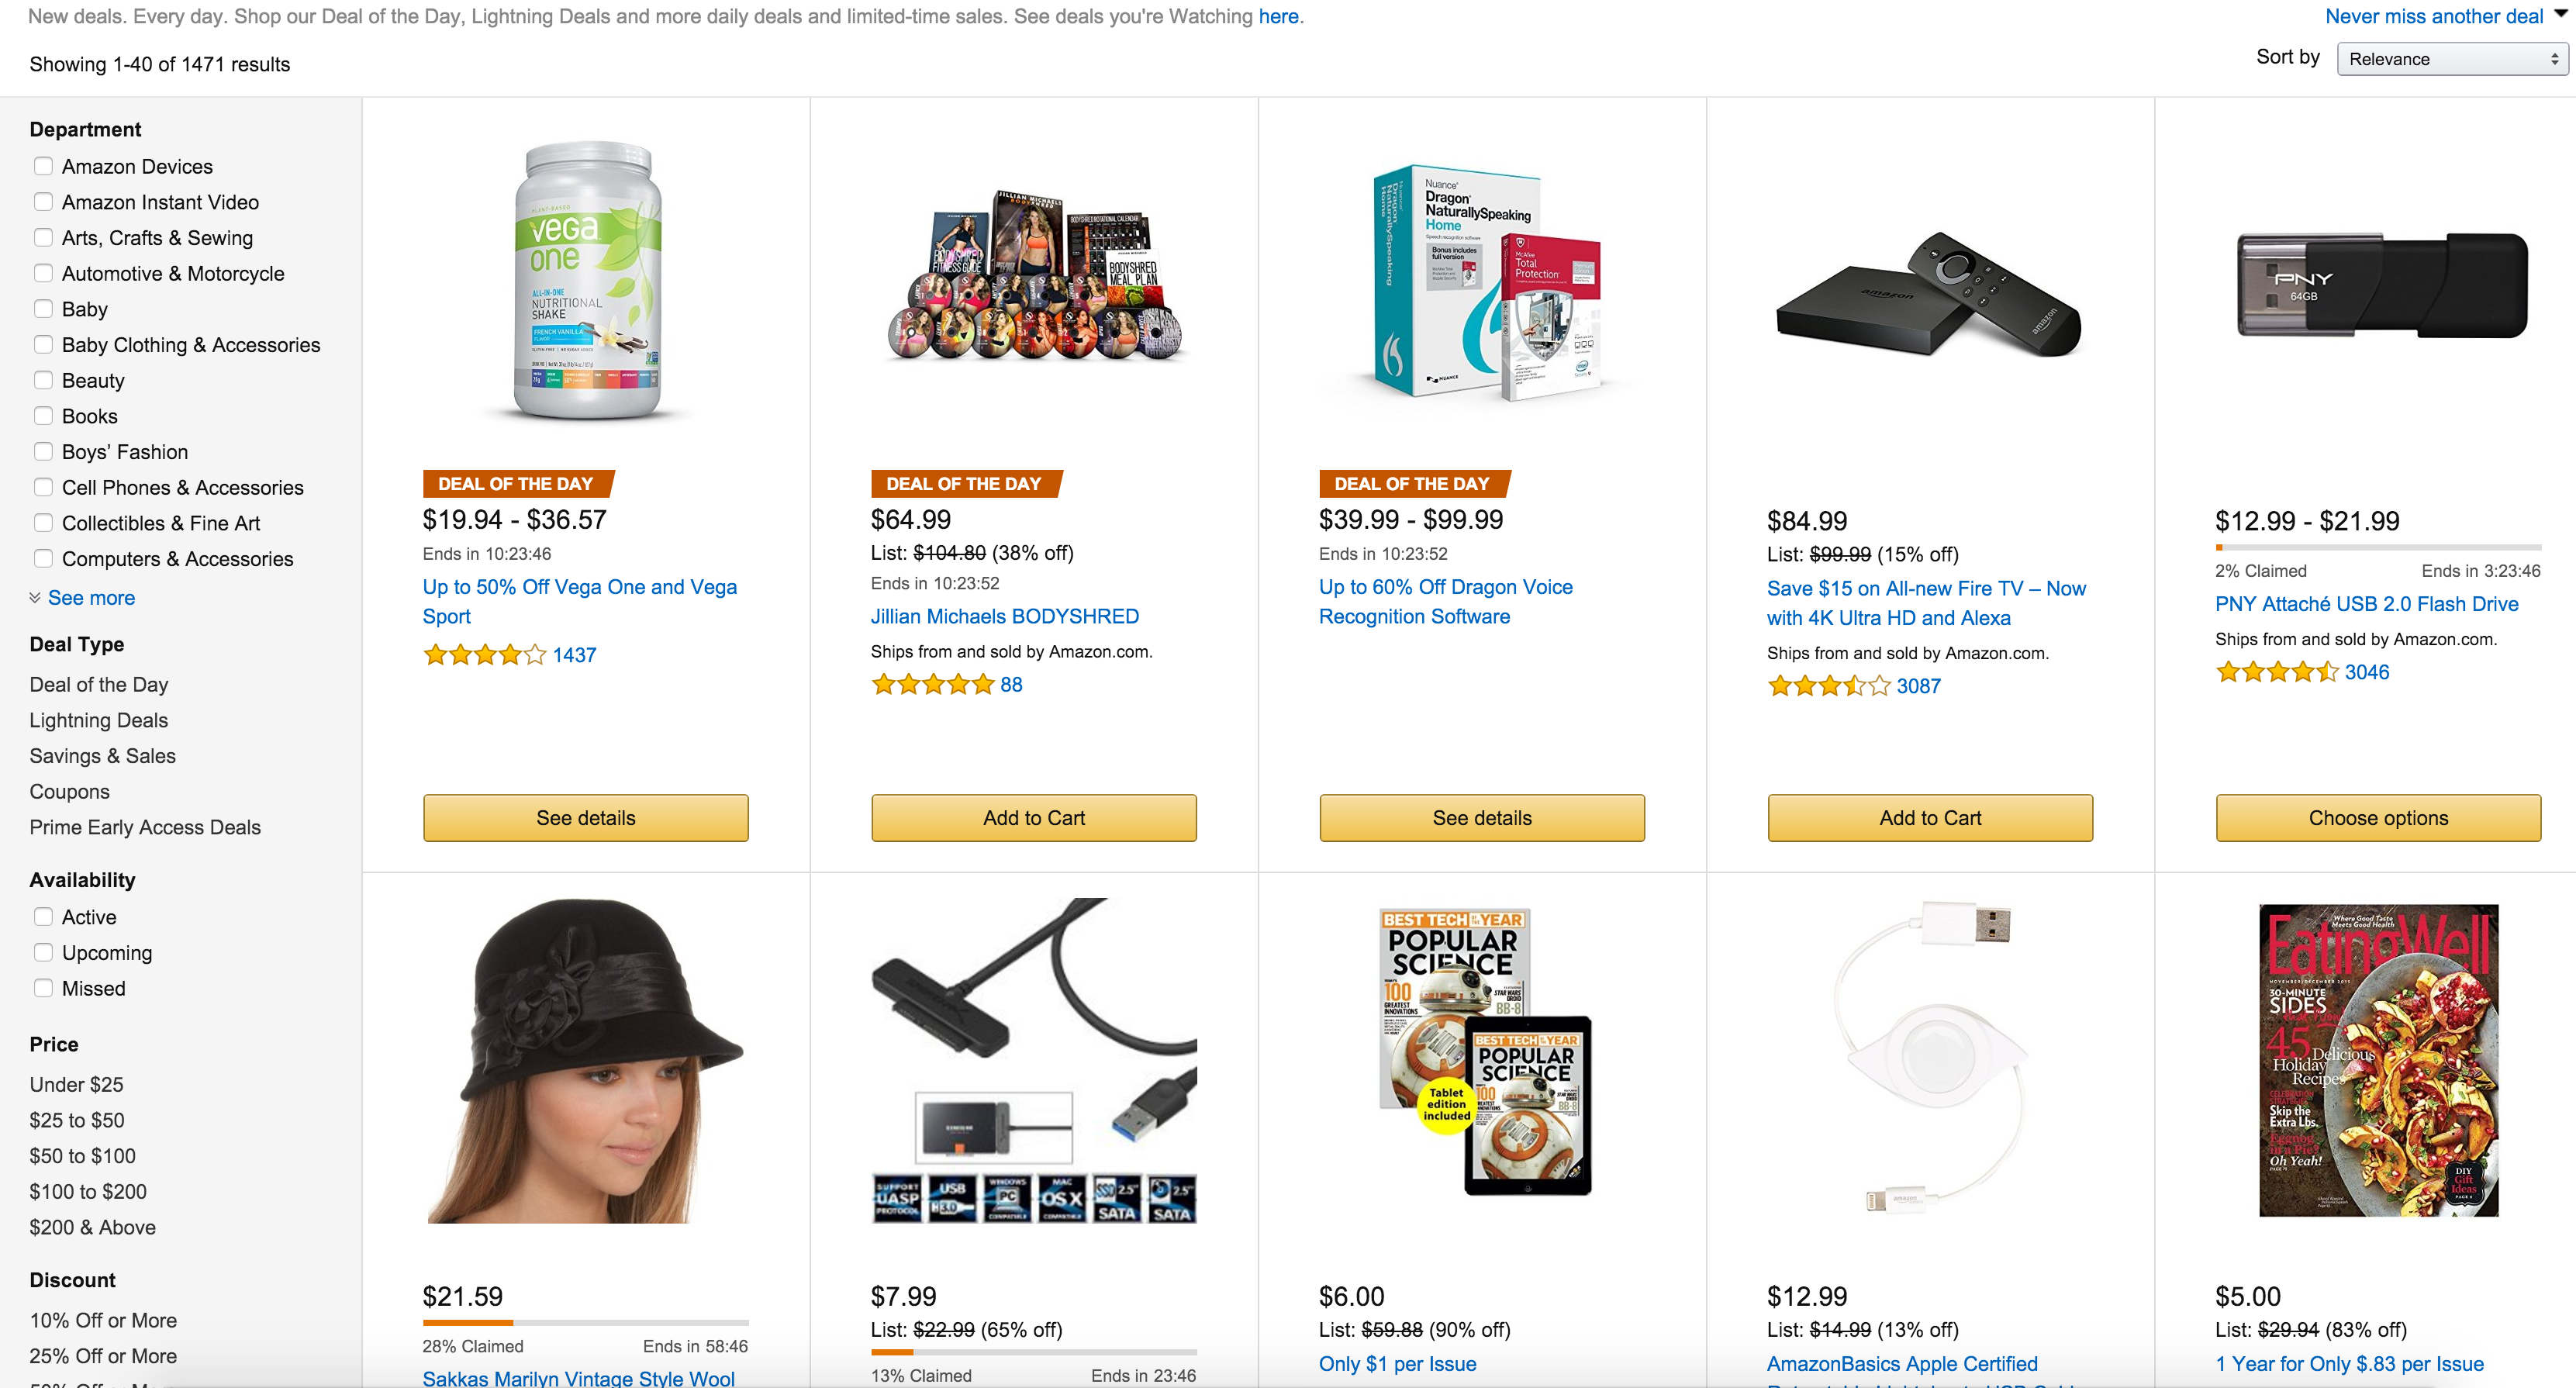
\includegraphics[width=1.0\linewidth]{images/chapter1/ex-amazon.png}\hfill
 \caption[Amazon shop]{Amazon shop}
 \label{fig:e_commerce_amazon_shop}
\end{figure}
The company was founded in 1994, spurred by what Bezos called his “regret minimization framework,” which described his efforts to fend off any regrets for not participating sooner in the Internet business boom during that time. In 1994, Bezos left his employment as vice-president of D. E. Shaw \& Co., a Wall Street firm, and moved to Seattle. He began to work on a business plan for what would eventually become Amazon.com.
Jeff Bezos incorporated the company as “Cadabra” on July 5, 1994. Bezos changed the name to Amazon a year later after a lawyer misheard its original name as "cadaver”. The company went online as Amazon.com in 1995.
\newline
Bezos selected the name Amazon by looking through the dictionary, and settled on “Amazon” because it was a place that was “exotic and different” just as he planned for his store to be; the Amazon river, he noted was by far the “biggest” river in the world, and he planned to make his store the biggest in the world. Bezos placed a premium on his head start in building a brand, telling a reporter, “There's nothing about our model that can't be copied over time. But you know, McDonald's got copied. And it still built a huge, multibillion-dollar company. A lot of it comes down to the brand name. Brand names are more important online than they are in the physical world.” Additionally, a name beginning with "A” was preferential due to the probability it would occur at the top of any list that was alphabetized.
\newline
Since June 19, 2000, Amazon's logotype has featured a curved arrow leading from A to Z, representing that the company carries every product from A to Z, with the arrow shaped like a smile.
\newline
After reading a report about the future of the Internet which projected annual Web commerce growth at 2,300\%, Bezos created a list of 20 products which could be marketed online. He narrowed the list to what he felt were the five most promising products which included: compact discs, computer hardware, computer software, videos, and books. Bezos finally decided that his new business would sell books online, due to the large world-wide demand for literature, the low price points for books, along with the huge number of titles available in print. Amazon was originally founded in Bezos' garage in Bellevue, Washington.
The company began as an online bookstore, an idea spurred off with discussion with John Ingram of Ingram Book (now called Ingram Content Group), along with Keyur Patel who still holds a stake in Amazon. In the first two months of business, Amazon sold to all 50 states and over 45 countries. Within two months, Amazon's sales were up to \$20,000/week. While the largest brick and mortar bookstores and mail order catalogs might offer 200,000 titles, an online bookstore could “carry” several times more, since it would have a practically unlimited virtual (not actual) warehouse: those of the actual product makers/suppliers.
Amazon was incorporated in 1994, in the state of Washington. In July 1995, the company began service and sold its first book on Amazon.com: Douglas Hofstadter's Fluid Concepts and Creative Analogies: Computer Models of the Fundamental Mechanisms of Thought. In October 1995, the company announced itself to the public.] In 1996, it was reincorporated in Delaware. Amazon issued its initial public offering of stock on May 15, 1997, trading under the NASDAQ stock exchange symbol AMZN, at a price of US\$18.00 per share (\$1.50 after three stock splits in the late 1990s).
\newline
Amazon's initial business plan was unusual; it did not expect to make a profit for four to five years. This “slow” growth caused stockholders to complain about the company not reaching profitability fast enough to justify investing in, or to even survive in the long-term. When the dot-com bubble burst at the start of the 21st century, destroying many e-companies in the process, Amazon survived, and grew on past the bubble burst to become a huge player in online sales. It finally turned its first profit in the fourth quarter of 2001: \$5 million, on revenues of more than \$1 billion. This profit margin, though extremely modest, proved to skeptics that Bezos' unconventional business modelcould succeed. In 1999, Time magazine named Bezos the Person of the Year, recognizing the company's success in popularizing online shopping.
\newline
Barnes \& Noble sued Amazon on May 12, 1997, alleging that Amazon's claim to be “the world's largest bookstore” was false. Barnes and Noble asserted, “[It] isn't a bookstore at all. It's a book broker.” The suit was later settled out of court, and Amazon continued to make the same claim.” Walmart sued Amazon on October 16, 1998, alleging that Amazon had stolen Walmart's trade secrets by hiring former Walmart executives. Although this suit was also settled out of court, it caused Amazon to implement internal restrictions and the reassignment of the former Walmart executives.

\subsection{Ebay}
Ebay Inc. is an American multinational corporation and e-commerce company, providing consumer to consumer \& business to consumer sales services via Internet. It is headquartered in San Jose, California. eBay was founded by Pierre Omidyar in 1995, and became a notable success story of the dot-com bubble. Today, it is a multibillion-dollar business with operations localized in over 30 countries.
\newline
The company manages eBay.com, an online auction and shopping website in which people and businesses buy and sell a broad variety of goods and services worldwide. In addition to its auction-style sales, the website has since expanded to include “Buy It Now” shopping; shopping by UPC, ISBN, or other kind of SKU (via Half.com); online classified advertisements (via Kijijior eBay Classifieds); online event ticket trading (via StubHub); online money transfers (via PayPal) and other services.
\newline
The website is free to use for buyers, but sellers are charged fees for listing items and again when those items are sold. The company also makes additional money through its PayPal subsidiary which is used by sellers to collect payment for items sold.
\begin{figure}[htb]
 \centering
 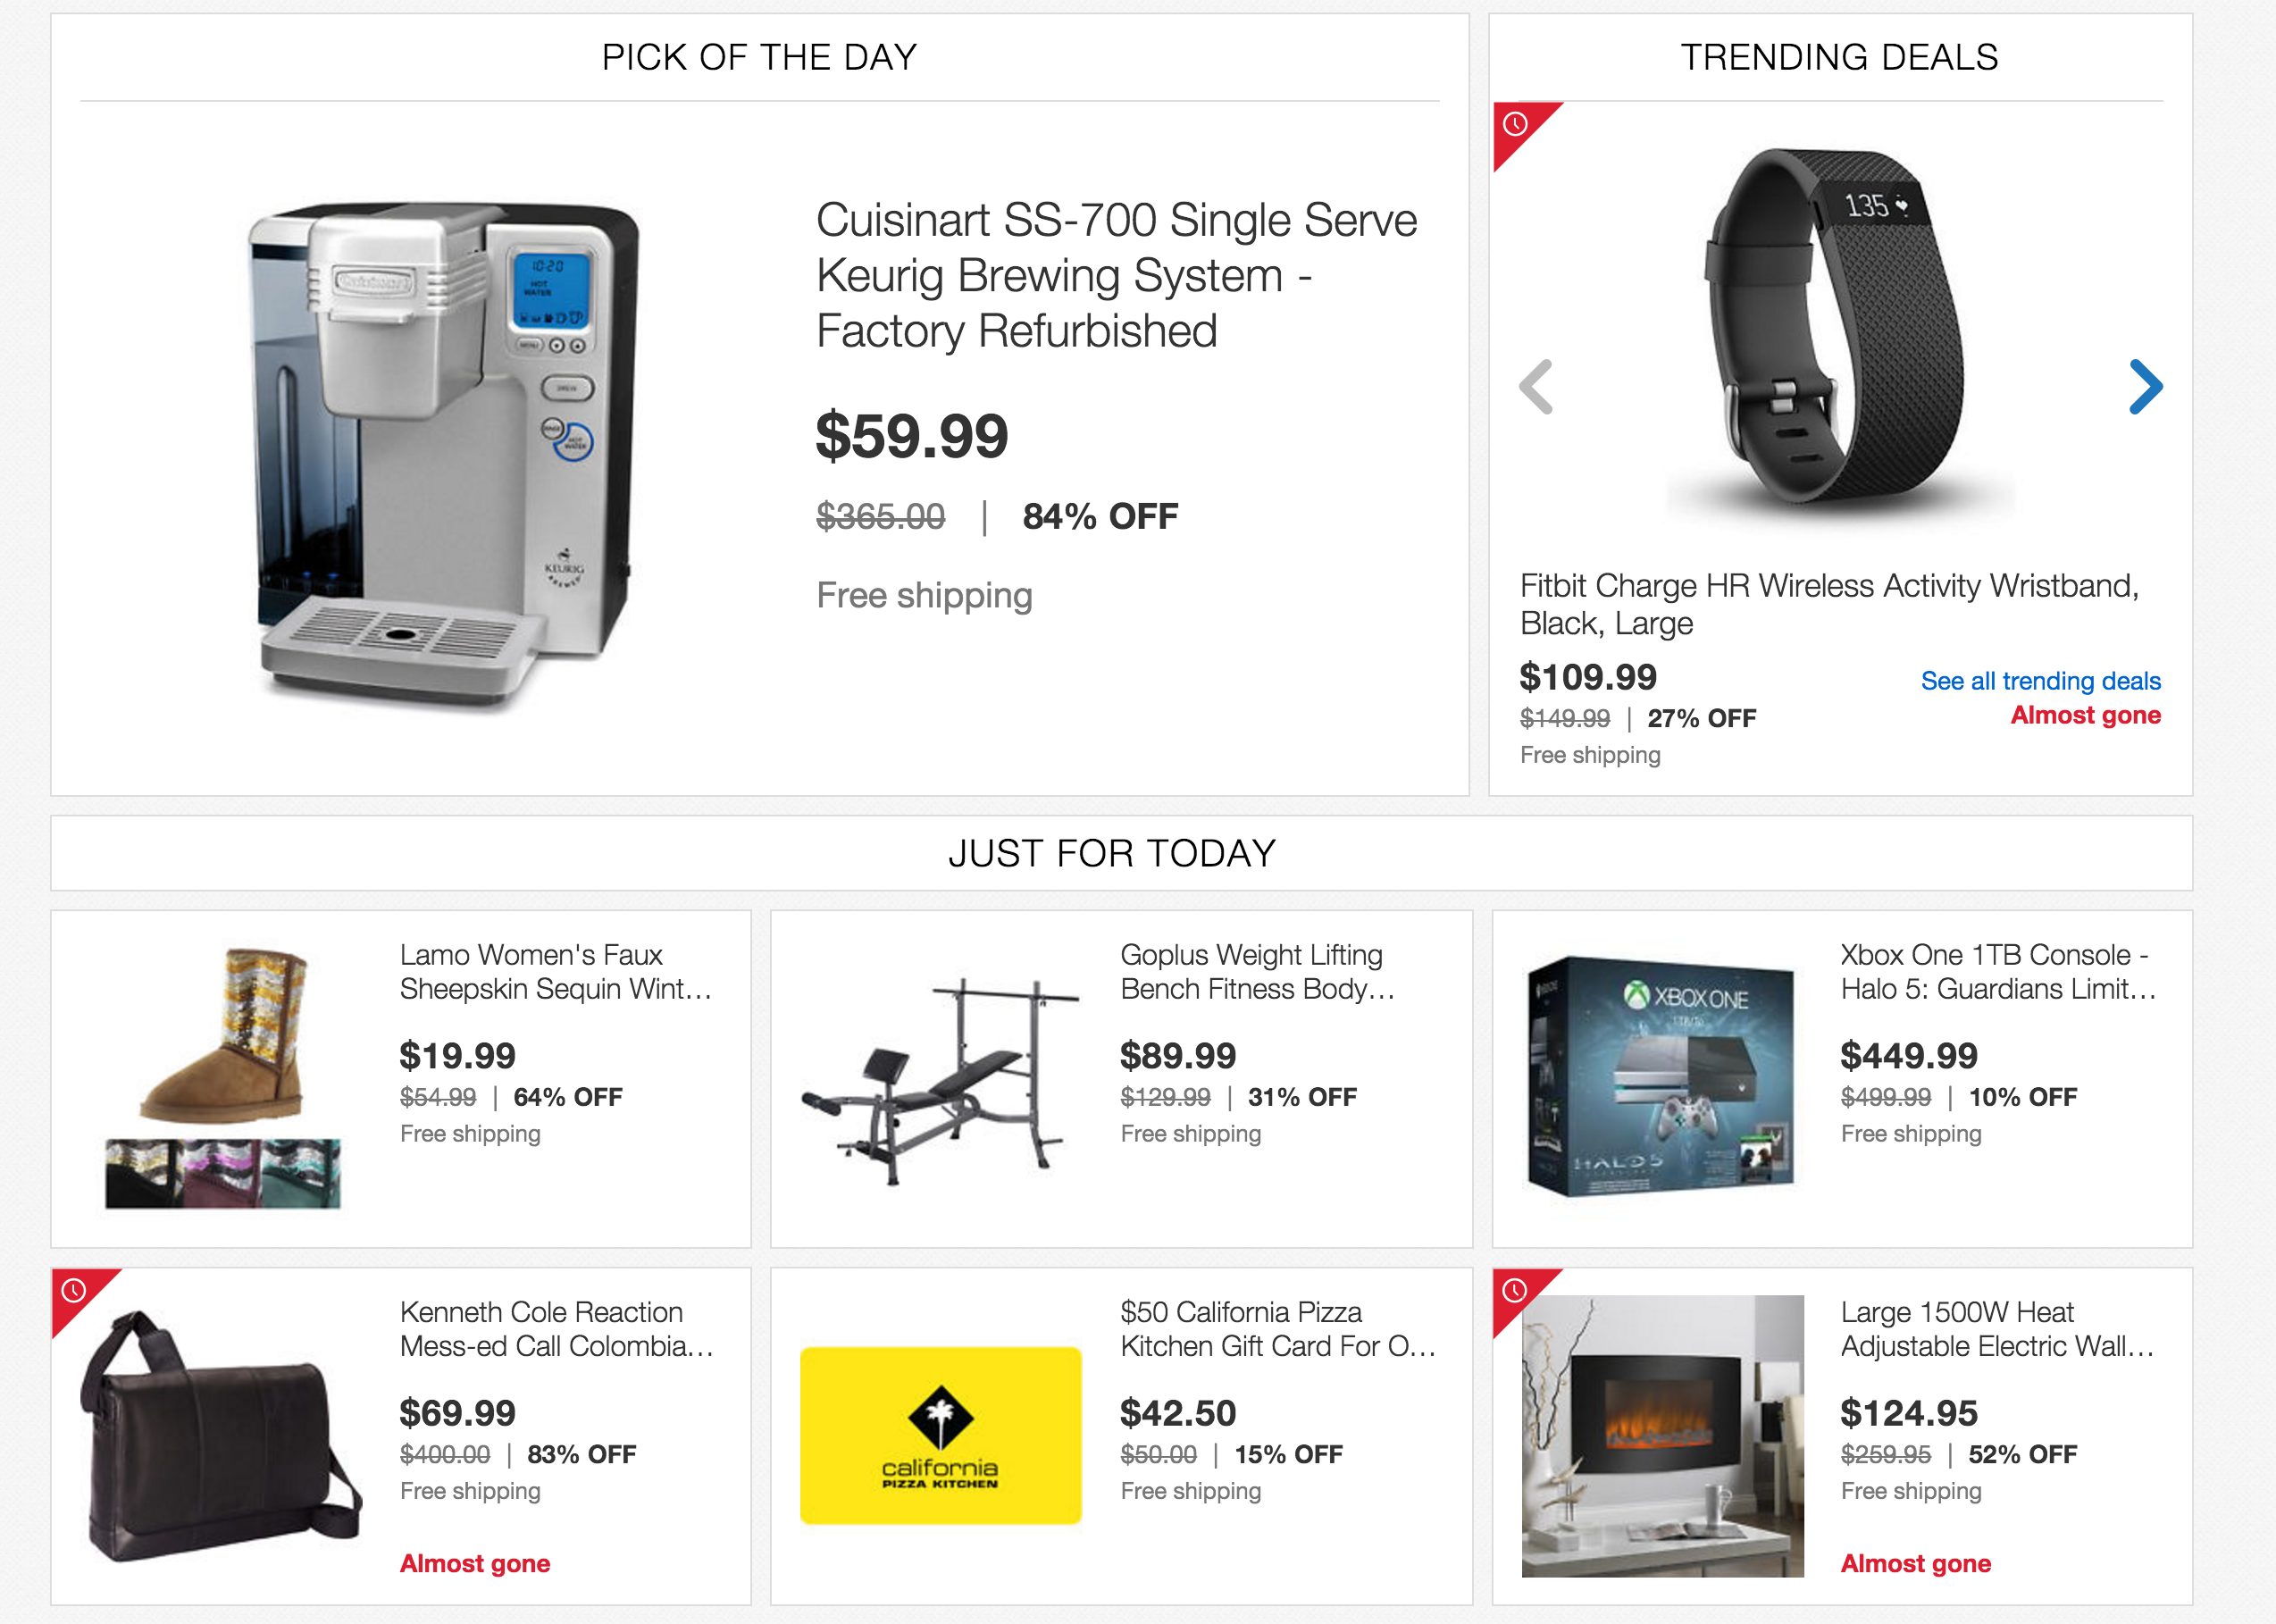
\includegraphics[width=1.0\linewidth]{images/chapter1/ex-ebay.png}\hfill
 \caption[Ebay shop]{Ebay shop}
 \label{fig:e_commerce_ebay_shop}
\end{figure}
AuctionWeb was founded in California, on September 4, 1995, by French-born Iranian-American computer programmer Pierre Omidyar (born June 21, 1967) as part of a larger personal site. One of the first items sold on AuctionWeb was a broken laser pointer for \$14.83. Astonished, Omidyar contacted the winning bidder to ask if he understood that the laser pointer was broken. In his responding email, the buyer explained: “I'm a collector of broken laser pointers.” The frequently repeated story that eBay was founded to help Omidyar's fiancée trade Pez candy dispensers was fabricated by a public relations manager in 1997 to interest the media, which were not interested in the company's previous explanation about wanting to create a “perfect market”. This was revealed in Adam Cohen's book, The Perfect Store (2002), and confirmed by eBay.
Reportedly, eBay was simply a side hobby for Omidyar until his Internet service provider informed him he would need to upgrade to a business account due to the high volume of traffic to his website. The resulting price increase (from \$30/month to \$250) forced him to start charging those who used eBay, and was not met with any animosity. It resulted in the hiring of Chris Agarpao as eBay's first employee to handle the number of checks coming in for fees.
Jeffrey Skoll was hired as the first president of the company in early 1996. In November 1996, eBay entered into its first third-party licensing deal, with a company called Electronic Travel Auction to use SmartMarket Technology to sell plane tickets and other travel products. Growth was phenomenal; in January 1997 the site hosted 2,000,000 auctions, compared with 250,000 during the whole of 1996. The company officially changed the name of its service from AuctionWeb to eBay in September 1997. Originally, the site belonged to Echo Bay Technology Group, Omidyar's consulting firm. Omidyar had tried to register the domain name echobay.com, but found it already taken by the Echo Bay Mines, a gold mining company, so he shortened it to his second choice, eBay.com.
In 1997, the company received \$6.7 million in funding from the venture capital firm Benchmark Capital.
Meg Whitman was hired as eBay President and CEO in March 1998. At the time, the company had 30 employees, half a million users and revenues of \$4.7 million in the United States.
eBay went public on September 21, 1998, and both Omidyar and Skoll became instant billionaires. eBay's target share price of \$18 was all but ignored as the price went to \$53.50 on the first day of trading.